\documentclass[review]{elsarticle}
\usepackage{lineno,hyperref}
\usepackage{syntonly}
\usepackage{geometry,amsmath,array}
\geometry{left=2.5cm,right=2.5cm,top=2.5cm,bottom=2.5cm}
\modulolinenumbers[5]

\journal{Journal of \LaTeX\ Templates}

%%%%%%%%%%%%%%%%%%%%%%%BBB
%% Elsevier bibliography styles
%%%%%%%%%%%%%%%%%%%%%%%
%% To change the style, put a % in front of the second line of the current style and
%% remove the % from the second line of the style you would like to use.
%%%%%%%%%%%%%%%%%%%%%%%

%% Numbered
%\bibliographystyle{model1-num-names}

%% Numbered without titles
%\bibliographystyle{model1a-num-names}

%% Harvard
%\bibliographystyle{model2-names.bst}\biboptions{authoryear}

%% Vancouver numbered
%\usepackage{numcompress}\bibliographystyle{model3-num-names}

%% Vancouver name/year
%\usepackage{numcompress}\bibliographystyle{model4-names}\biboptions{authoryear}

%% APA style
%\bibliographystyle{model5-names}\biboptions{authoryear}

%% AMA style
%\usepackage{numcompress}\bibliographystyle{model6-num-names}

%% `Elsevier LaTeX' style
\bibliographystyle{elsarticle-num}
%%%%%%%%%%%%%%%%%%%%%%%

\begin{document}

\begin{frontmatter}

\title{An energy-efficient approach for budget-constrained tasks in mobile cloud computing}
\tnotetext[mytitlenote]{Fully documented templates are available in the elsarticle package on \href{http://www.ctan.org/tex-archive/macros/latex/contrib/elsarticle}{CTAN}.}

%% Group authors per affiliation:
\author{Elsevier\fnref{myfootnote}}
\address{Radarweg 29, Amsterdam}
\fntext[myfootnote]{Since 1880.}

%% or include affiliations in footnotes:
\author[mymainaddress,mysecondaryaddress]{Elsevier Inc}
\ead[url]{www.elsevier.com}

\author[mysecondaryaddress]{Global Customer Service\corref{mycorrespondingauthor}}
\cortext[mycorrespondingauthor]{Corresponding author}
\ead{support@elsevier.com}

\address[mymainaddress]{1600 John F Kennedy Boulevard, Philadelphia}
\address[mysecondaryaddress]{360 Park Avenue South, New York}

\begin{abstract}
    Despite significant technological advancements in recent years, Smart Mobile Devices (SMDs) are still low potential computing devices owing to its limited battery life. Therefore, it will makes sense to offload heavy mobile applications tasks to more powerful machines in the cloud.
    In this paper, we introduce a 3-layer architecture architecture that includes a Central Resource Broker (CRB),which Consists of a few computers ,sitting between local mobile cloud (volunteer computing systems ) and remote cloud like EC2 ,Amazon,etc.The CRB is decision maker based on the results of CRO scheduling strategy mentioned above.Based on the architecture mentioned above,we then propose a computation scheduling technique to offloading the outsourced tasks to achieve the target at reducing the energy consumption on mobile and monetary expenditure of the CRB.
    Experimental results of simulations demonstrate the effectiveness of the 3-layer architecture and the efficiency of the proposed method. Moreover, compared to standalone mobile or cloud execution,The mobile devices can archive reduction in power consumption and total cost on purchase the computing service provided by the cloud infrastructure ,by XX\% and XX\% ,respectively ,compared with baseline methods .
\end{abstract}

\begin{keyword}
    \texttt {}mobile cloud computing \sep  {energy efficient} \sep {budget-constrained}
    \MSC[2010] 00-01\sep  99-00
\end{keyword}

\end{frontmatter}

%%\linenumbers

\section{Introduction}
In summary, this paper makes the following contributions:
\begin{itemize}
    \item We propose a new system architecture for mobile cloud computing that include 3 layer , the first one is the local cloud organized by the smart  mobile devices(SMDs),these SMDs can volunteer to provide its resource to nearby peers ,and use the resource it lack and nearby device can provide.the second layer is called Central resource Broker (CRB),sitting between mobile devices and remote cloud infrastructure .The third one is the remote cloud like EC2 ,Amazon.

    \item  we propose a novel algorithm to help SMDs to decide the destination to offload its task ,local P2P-based cloud environment or remote cloud infrastructure to reduce energy consumption and the monetary cost constrained by the budget defined by the user . And it was proved to be efficient  through extensive simulations.
\end{itemize}

\paragraph{}% paper  organized
    The rest of this paper is organized as follows: Section 2 includes the related works. Section 3 presents the 3-layer architecture we proposed . The heuristic algorithm is introduced in Section 4 . Section 5 describes the performance evaluation of the proposed tasks scheduling system. . Conclusions are drawn and future work is discussed in the last section.

\section{Related work}
\section{Problem definition}
     \subsection{Local Execution}

\section{System Model Description}
    \paragraph{}
    The novel system architecture for MCC including three layer is shown in Fig\ref{fig:architecture}. The first layer is the local clouding computing system organized by the smart mobile devices(SMDs),these SMDs can volunteer to provide its resource to nearby peers,and use the resource it lack but nearby device can provide.After that,the second layer is called Central resource Broker (CRB),sitting between mobile devices and remote cloud data center.Then The third one is the remote cloud infrastructure like EC2 ,Amazon,providing cloud computing service and charging some fee for every processing request according to certain rules,like resource usage amount or processing time.
    \paragraph{}
    The CRB plays a significant part in the system architecture to extend the the SMD's battery life.On the one hand,the CRB maintains a list of resource in local environment reported by each SMD at the very beginning of every scheduling period.when received a task processing request,the CRB schedule the task either in a local or remote way.On the other hand,when a task can not be executed in local cloud ,the CRB purchase the remote cloud service to complete the task.Above all,the CRB is a decision maker in our proposed system,though it don't process the task in CRB itself.This approach greatly reduce the possibility of the occurrence of single node failure


\begin{figure}[ht]
\centering
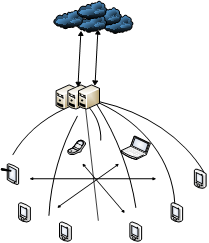
\includegraphics[scale=0.7]{architecture.png}
\caption{Proposed system architecture}
\label{fig:architecture}
\end{figure}

\section{Theoretical Model}
        \paragraph{}
        In this section,we introduce the theoretical model of our proposed mobile cloud computing system.We consider a set of mobile device user are located near to each other and each of which can either be a offloading destination or has a computationally intensive and delay sensitive task to be completed and get result send back.The set of neighbouring devices are represented by
        $$N=(n_{1},n_{2},...,n_{m})$$
        \paragraph{} Considering the tasks submitted by the local SMD,we denote $J=(j_{1},n_{2},...,j_{x})$ as a set of task,and each task $j_{i}$ can be represented by a tuple$j_{i}=(T_{datasize}^i,T_{deadline}^i) $ where the datasize and deadline are denoted as the data need to be transmitted and max latency can be tolerated by user for the task $i$,respectively.
         \paragraph{} Our approach for energy-optimal application execution is to choose where to execute the task,with an aim to tremendously reduce the average energy consumed on all the devices in local clouding computing system.Therefore,the energy consumed by local devices to offloading their task to local device or remote cloud server need to be compared and produce a tradeoff through our proposed alogrithm.let $x$ represent the offloading decision the CRB make,when the task is executed on a local device,$x=0$,otherwise,the $x$ will be set to 1.
               $$\begin{cases}
               {\epsilon_{mob}^i}<{\epsilon_{cld}^i} & x = 0\\
               {\epsilon_{mob}^i}\geq{\epsilon_{cld}^i} & x = 1\end
               {cases}$$
         where the $\epsilon_{mob}^i $ and  $\epsilon_{cld}^i $ are denoted as energy cost on mobile device and remote cloud respectively for a single task.
        \subsection{Energy Model}
            Now we define $T_{cyc}^i$ as the number of instructions needed to execute a task for a given data size of $T_{datasize} $,and $T_{cyc}$ can be calculated by the formula below :\\
            $$ T_{cyc} = X\cdot T_{datasize} $$
            where the $X$ is a coefficent with an emprirical distribution\citep{lorch2001improving} and depend on the nature of the application.and the relationship between the number of CPU cycles and bit follows a Gamma distribution\citep{lorch2001improving}.
            For a given Application completion probility(ACP) $\rho$ that a task $j_i$ can meet its deadline $T_{deadline}^i$ using $W_{\rho} $ CPU cycles,the number of
            CPU cycles needed is expressed as :\\
            $$W_{\rho}=F_{W}^{-1}(\rho)=LF_{X}^{-1}(\rho)$$
            where $F_{W}(W_{\rho})={\rm P}[w\leq W_{\rho}]\geq\rho$ \cite{wen2012energy},which is the Formula quantile for the distribution of Formula.

            \subsubsection{cloud Execution Energy Model}
             \noindent When the application is executed on the remote cloud server,the energy consumed by the mobile device primarily depend on the amount of data to be transmitted from the device to the remote cloud server.we assume that there is a stochastic fading model for the wireless channel between mobile device and remote cloud,which is characterized by a channel gain of $g$ and a noise power of $ N$.Here we adopt the Gilbert-Elliott(GE) channel model\citep{zafer2007minimum},which is widely known and used.There aer two channel conditions:good and bad ,denoted as G and B,respectively.When the measured channel gain is above some value,the channel is labeled as good.Otherwise,the channel is labeled as bad.The average channel gains of the good and bad states are denoted as  $g_{G}$ and  $g_{B}$,respectively.The state transition matrix is as follows: \\
             $$P=\begin{bmatrix}P_{GG} & P_{GB} \\P_{BG} &P_{BB} \end{bmatrix}$$

          %   We assume that the transmission power on mobile device is a constant value,
             \noindent For a task $j_{i}=(T_{datasize}^i,T_{deadline}^i)$ ,it has  $T_{datasize}^i$ bits data need to be transmitted to cloud server.As a result ,the total energy consumption on the source device for cloud execution is $\epsilon_t(s_t,\bar{g_t},n)$ where $s_t$
             and $g_t$ are the size of data in transmission and channel state in time slot $t$ ,respectively.The energy consumed to transmit $s_t$ bits data over a fading wireless channel with a gain of $g$ ,at time slot index of $t$ ,is a convex monomial function given by
             $${\cal E}_{t}(s, g, n)=\lambda{s^{n}\over g},\eqno{\hbox{(3)}}$$
             where $n$ denotes the monomial order,and $\lambda$ denotes the energy coefficient \citep{zafer2007minimum,neely2005dynamic}.Generally,It is often assumed that $2\leq n\leq5$, depending on the modulation scheme.According to the measurements in \citep{miettinen2010energy}we set $\lambda=1.5$.

            \subsubsection{Mobile Execution Energy Model}
             When the task is offloaded to nearby device as a destination,the total energy consumption incorporate two parts,the first part is energy spent on communication for both transmission and reception of the data,the other part is determined by the CPU workload of the destination device,which is measured by the number of CPU cycles required by the application,denoted as W.
             \paragraph{} We assume that $ f $ is the clock frequency of the chip ,which is approximately linearly proportion to the voltage of $ V $ supply to the chip .However,the energy consumption cab be substantially reduced by optimally configuring the clock frequency of the chip by DVS\citep{rabaey2002digital}.And In the CMOS circuits\citep{wen2012energy} ,the energy cost on a single operation $ \epsilon_w $ is proportional to $ {v^2} $.In consequence,the energy cost by a operation can be represented by ,\\
             $$ \epsilon(f)=\kappa\cdot{f^2}$$.
             where $kappa $is the coefficient depending on the chip architecture.According to the measurements in \citep{miettinen2010energy} ,we set $kappa=10^{-11}$ here.
             \paragraph{}In order to save energy of the executing device,the optimal clock scheduling approach can be represented as \\
             $$f^{\ast}(w)={\theta\over T^{'}[F_{W}^{c}(w)]^{1/3}}$$
             where the $\theta=\sum_{i=1}^{W_\rho}[F_W^c(i)]^{\frac{1}{3}} $ and $T^{'}=T_{deadline}-\frac{T_{datasize}}{R(x)}$.
             \paragraph{}
             With the optimal transmission policy\citep{wen2012energy},the minimum expected energy cost $\eqalignno{{\cal E}_{c}^{\ast}} $ to tansmitted $L$ bits data is given by: \\
             $$  \eqalignno{{\cal E}_{c}^{\ast}(T_{datasize}, T_{dealine}) &= {T_G\over T_{G}+T_{B}}{\cal E}_{t}(T_{datasize};G) \cr &+ {T_B\over T_{G}+7_{B}^{\gamma}}{\cal E}_{t}(T_{datasize};B) } $$
             where ${\cal E}_{t}(L;G)$ and ${\cal E}_{t}(L;B)$ represent the mnimum expected energy cost when the channel is in good and bad state,respectively,and they can be expressed as :\\
             $${\cal E}_{t}(T_{datasize};G)=\lambda L^{n}\zeta_{t;G} $$
             $${\cal E}_{t}(T_{datasize};B)=\lambda L^{n}\zeta_{t;B} $$
             % \paragraph{}In this paper ,we task the baseline power consumption $ \epsilon_{idle}$ into consideration which means the energy cost when the device is idle.As such,
             %We set Formula so that energy consumption is consistent with the measurements in ""Energy efficiency of mobile clients in cloud computing""

        \subsection{Response Time Model}
            \subsubsection{cloud computing}
            \paragraph{} specifically,every task is assigned a maximum response time that should not be exceeded ,otherwise,the satisfactory quality of experience(QoE) would not be provided to the application user.the deadline of a task must be taken into consideration when it comes to the decision on whether offloading or not,additionally ,where to offloading.
            \paragraph{} In the case of offloading to a neighbouring SMD,the response time
            \paragraph{} However,In the case of offloading to a server of remote data-center,the composition of the response time become more complicated as the latency have to incorporate the time to transmitting the input data to remote server ,to executing on the server and result sent back to the SMD .More specifically, the minimum time $ T_{tk} $ necessary to transmit $ N_{k} $ bits of duration $ T_{b} $ over an additive white Gaussian noise (AWGN) channel is  \\
            $$T_{tk}={N_{k}T_{b}\over \log_{2}\left(1+{p_{tk}\vert H_{k}\vert ^{2}\over \Gamma({\rm BER}_{{\rm k}})d_{k}^{\beta}N_{0}}\right)}, \eqno{\hbox{(1)}}$$
            where $ P_{tk} $ is the transmit power of the $k$-th SMD. \citep{barbarossa2013joint} \\
            \paragraph{} In practice,The average delay associated to the correct reception of Formula bits at the server side, incorporating packet duration and retransmissions, is then \\
            $$\Delta_{tk}=\bar{S} _{k}T_{tk}={N_{k}T_{b}\over (1-P_{ek})\log_{2}\left(1+{p_{tk}\vert H_{k}\vert ^{2}\over \Gamma({\rm BER}_{k})d_{k}^{\beta}N_{0}}\right)}. \eqno{\hbox{(2)}}$$
            To summary the overall (average) latency when the task offloading from SMD to a remote server ,we give the following expression :\\
            $$L_{k}^{\prime}=\Delta_{tk}+{w_{k}\over f_{k}}+T_{rk} \eqno{\hbox{(3)}}$$

            \subsubsection{local computing}
            For the local computing approach,a mobile device user executes its computation task locally on the nearby resource-providing device.let $ \mu_{mob}$ be the computation capability of the destination device in MIPS.In practice,the computation capability may differ from device to device.Therefore ,the execution time of the task $ i$ by mobile device k in local mobile cloud computing environment is then given as \\
            $$ t_{local}^j = \frac{{T_{datasize}^i}+R_{datasize}^i}{BW_{local}}+\frac{T_{ins}}{\mu_{mob}}$$
            where $R_{datasize}^i$ is denoted as the data of execution result received by the mobile device user.

        \subsection{Performance metric}
        \subsection{Workload model}
        The inter-arrival time and request size have a Weibull distribution while the request duration follows a Normal distribution.\cite{iosup2008performance}
        \section{Performance evaluation}
            \subsection{Simulation set-up}
            \paragraph{}
            %we adopted the results in [19] where the ratio of energy consumption between 3G and ad hoc WLANs was 20/1 without a specific unit.\cite{ristanovic2011energy}
\section{Dynamic offloading algorithm}
    \subsection{Decision-making on offloading destination selection }
    \paragraph{}
    Now we are address more on the question of dynamically scheduling the tasks to be executed either locally or remotely ,with a aim to augment the capability and prolong the battery life.
    \paragraph{}
     Now we both consider the energy and cloud service purchsing cost under the constrain of each task's deadline,and the optimization problem can then be cast as below:\\
      objective: $\alpha \cdot \frac{\sum_{i=0}^{\parallel n\parallel}E_{mob}^i}{\parallel n \parallel} + \beta \cdot \frac{ m}{\parallel J\parallel}$\\
      subject to: $ frac{c_{j}}{log_{2}{(1+p_{j}a_{j})}} +frac{W_{j}}{mu_{cld}} leq T_{deadline}^{j} , forall j_{1},j_{2},...,parallel Jparallel$ \\
    where $c_{j} =\frac{T_{datasize}^j \cdot t_b\cdot \log2}{(1-p_{ek})}  $ and $ a_j=\frac{  \vert H_{k}\vert ^{2}}{\Gamma({\rm BER}_{{\rm k}})d_{k}^{\beta}N_{0}} $.
    \paragraph{}
\section{Performance Evaluation}
\subsection{simulation set-up}
\paragraph{} In this section,we conduct several simulations to evaluate the performance of the proposed MCC system and the offloading algorithm. The effectiveness and efficiency of our approach were evaluated mainly in terms of the the radio the violation of QoS and the average energy consumption by a mobile device. Comparisons were made .....%among the following three scenarios:
\subsection{Assumptions and parameters}
Besides,In our simulation experiment,we assume that the SMDs are motionless, staying in their positions uniformly distributed in a fixed rectangular area,\cite{vellore2009performance},because the effect of mobility of SMDs may violate the assumptions,and the mobility will be considered in our future work.we further assume the number of tasks generated by the local devices at each time slot follows Binomial distribution with parameter$f$.
\paragraph{}
In our simulated cloud environment,we fairly assume that the computational power(MIPS) of the remote server and that of mobile device are XX and XXX respectively.
%In our simulated cloud environment ,we fairly assume that the computational power(MIPS) of the remote server is double that of the mobile device ,and the size of both of them is fixed throughout. We choose a mobile device speed of 500 MIPS ,but 1000 MIPS for  remote hos in remote cloud environment. Besides , we assume that maximum bandwidth of the wireless network for mobile device to connect to CRB 300Mbit/s ,because the CRB is located next to WIFI Aps.
\subsection{Performance metric}
\section{Conclusion and future work}
\section{Acknowledgment}
\section*{References}

\bibliography{mybibfile}

\end{document}
